\documentclass{article}      % Specifies the document class

%encoding
%--------------------------------------
\usepackage[ddmmyyyy]{datetime}
%--------------------------------------

%encoding
%--------------------------------------
\usepackage[utf8]{inputenc}
\usepackage[T1]{fontenc}
%--------------------------------------

%colors
%--------------------------------------
\usepackage[usenames, dvipsnames]{color}
%--------------------------------------


%images
%--------------------------------------
\usepackage{graphicx}
%--------------------------------------

%Header and footer commands
%--------------------------------------
\usepackage{lastpage}
\usepackage{fancyhdr}
%--------------------------------------

%%%%%%%%%%%%%%%%%%%%%%%%%%%%%%%%%%%%%%%
%ALTERAR AQUI A VERSÃO DO DIGESTOR!!!!!
\newcommand{\versiondigester}{v1.0.1.0}
%%%%%%%%%%%%%%%%%%%%%%%%%%%%%%%%%%%%%%%

%Header and footer commands
%--------------------------------------
\pagestyle{fancy}
\fancyhf{}
\rhead{Digester \versiondigester}
\lhead{Yandeh}
\lfoot{Yandeh}
\rfoot{\today}
\fancyfoot[C]{\footnotesize Página \thepage\ de \pageref{LastPage}}

\fancypagestyle{firststyle}
{
   \fancyhf{}
   \rhead{Digester \versiondigester}
   \lhead{Yandeh}
   \lfoot{Yandeh}
   \cfoot{Página \thepage}
   \rfoot{\today}
   \fancyfoot[C]{\footnotesize Página \thepage\ de \pageref{LastPage}}
}

%Portuguese-specific commands
%--------------------------------------
\usepackage[portuguese]{babel}
%--------------------------------------

%Hyphenation rules
%--------------------------------------
\usepackage{hyphenat}
\hyphenation{mate-mática recu-perar}
%--------------------------------------

\title{Release Notes \\
      Digester \versiondigester}  % Declares the document's title.
\author{Yandeh Team}              % Declares the author's name.
\date{São Paulo, \today}       

\begin{document}             % End of preamble and beginning of text.

\maketitle                   % Produces the title.

\thispagestyle{firststyle}


\begin{table}[!ht]
\centering
\caption{Histórico de atualizações}
\label{my-label}
\begin{tabular}{|l|l|l|l|}
\hline
\textbf{Versão} & \textbf{Data} & \textbf{Descrição}                & \textbf{Autor}                                       \\ \hline
1.0.0.0           & 22/06/2016    & Revisão Inicial                 & Danilo Guanabara                                     \\ \hline
1.0.0.1           & 27/06/2016    & Bugfixes                        & Danilo Guanabara                                     \\ \hline
1.0.0.2           & 30/06/2016    & Bugfixes e limpeza              & Rosemary Sumitani                                    \\ \hline
1.0.0.3           & 04/07/2016    & Testes Unitários, bugfixes      & Danilo e Rosemary                                    \\ \hline
1.0.0.4           & 07/07/2016    & Parser Daruma, Bugfixes         & Luis, Danilo e Rosemary                              \\ \hline
1.0.0.5           & 17/07/2016    & Bugfixes Parser Daruma          & Luis Sant'Ana                                        \\ \hline
1.0.0.6           & 14/07/2016    & BugFixes Parser Daruma          & Luis Sant'Ana                                        \\ \hline  
1.0.0.7           & 18/07/2016    & BugFixes Troca Impressoras      & Luis e Danilo                                        \\ \hline
1.0.0.8           & 29/07/2016    & Bugfixes                        & Yandeh Team                                          \\ \hline
1.0.0.9           & 01/08/2016    & Parser SAT                      & Luis Sant'Ana                                        \\ \hline
1.0.1.0           & 04/08/2016    & Bugfixes                        & Luis Sant'Ana                                        \\ \hline
\end{tabular}
\end{table}



\section{Objetivos}

Este documento tem o objetivo de descrever as alterações nas funcionalidades do Digester para a versão \versiondigester. 


\section{Introdução}     
Nesta versão foi realizado correções encotradas durante o processamento de dados advindos de equipamentos ECF e SAT. Do grupo de ECFs apenas foram corrgidas problemas encontrados nos modelos Daruma e Epson.

\section{O que mudou?}

Nenhuma novidade em relação à versão anterior, apenas correções de \emph{bugs}.


\begin{figure}[!ht]
  \centering
    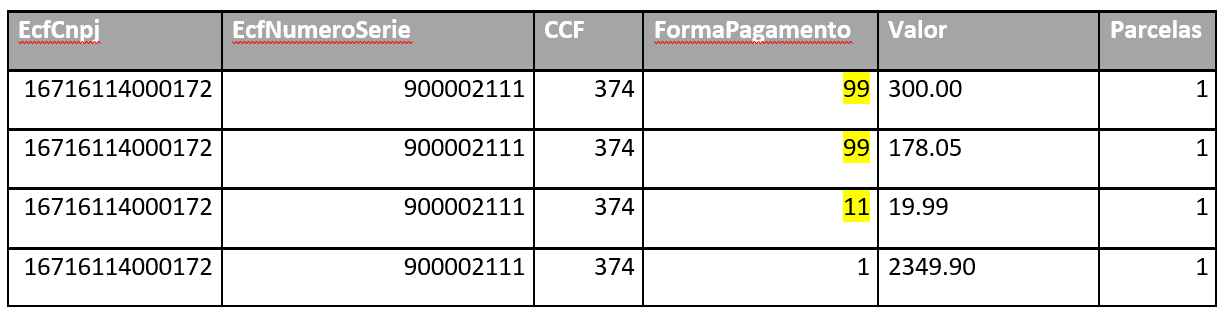
\includegraphics[width=1.0\textwidth]{tabela.PNG}
    \caption{Erro evidenciado}
    \label{fig:tabela}
\end{figure}

\begin{figure}[!ht]
  \centering
    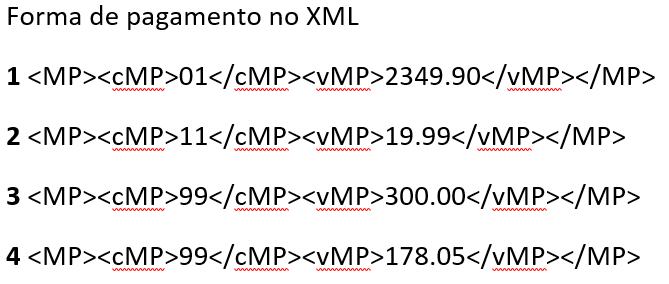
\includegraphics[width=0.8\textwidth]{cml.PNG}
  \caption{Trecho do XML com os códigos de pagamento e valores}
  \label{fig:xml}
\end{figure}

\subsection{Correções}

\subsubsection{SAT}
\begin{itemize}
\item ConsumidorCpfCnpj – Não está sendo apresentado. Correção realizada através da correta captura da tag no arquivo XML.
\item CupomValorDesconto - Não está apresentando o valor do desconto. Correção realizada através da correta captura da tag no arquivo XML.
\item ItemCodigo – Está mostrando um número a mais no código. O campo no arquivo XML está vindo um dígito a mais, o problema provavelmente está associado ao software frente caixa e impressora, que não imprime o último digito no cupom fiscal.
\item ItemValor – O campo ItemValor está sendo apresentado o valor final do item. Correção realizada capturando a tag vUnCom.
\item FormaPagamento – Não está apresentando o código de pagamento correto. Na figura \ref{fig:xml} está o trecho do arquivo XML que apresenta as formas de pagamento utilizadas da figura \ref{fig:tabela}. Note que é realizada a captura da forma correta, o que sugere que o problema está relacionado a identificação da forma de pagamento, um problema do software de frente de caixa de classifica o tipo de pagamento de forma errada. A seguir está a identificação de cada código de pagamento extraído do manual de especificação técnica de requisitos do SAT~\cite{sat}: 

\begin{itemize}
\item 01 - Dinheiro
\item 02 - Cheque
\item 03 - Cartão de Crédito
\item 04 - Cartão de Débito
\item 05 - Crédito Loja
\item 10 - Vale Alimentação
\item 11 - Vale Refeição
\item 12 - Vale Presente
\item 13 - Vale Combustível
\item 99 - Outros
\end{itemize}

\item Valor – Não mostra o valor após o desconto do cupom. Correção realizada através da correta captura da tag no arquivo XML.
\end{itemize}

\subsubsection{Daruma}
\begin{itemize}
\item FormaPagamento – Não está apresentando no código de pagamento Unknown. Correção realizada alterando o comando de abertura de pagamento.
\item Os cupons que tem pagamentos realizados em mais de uma forma um dos valores vem zerados ou Unknown. A correção do item anterior resolveu também este item.
\end{itemize}

\subsubsection{Epson}
\begin{itemize}
\item ConsumidorCpfCnpj – Em um dos cupons não está sendo apresentado o CPF do consumidor. Neste cupom em especial o campo CPF veio vazio.
\item O COO não é o mesmo gerado no Cupom impresso. Este problema é um problema persistente das impressoras Epson, detalhado no realease notes da versão 1.0.0.7.
\item Existe uma venda que não foi efetuada. Problema no arquivo de coleta, este arquivo termina no meio de uma venda e não há arquivo na sequência.
\end{itemize}

\section{Limitações}
Nenhuma limitação a princípio.

\section{Como funciona?}

Dentro da estrutura de arquivos (/home/hadoop/Coleta/) existe um arquivo chamado $processa\_genericos.py$, onde pode ser editado o seguinte trecho em amarelo, indicando a faixa de dias a serem processados e o trecho em verde indica o ano e mês.

\begin{figure}[!ht]
  \centering
    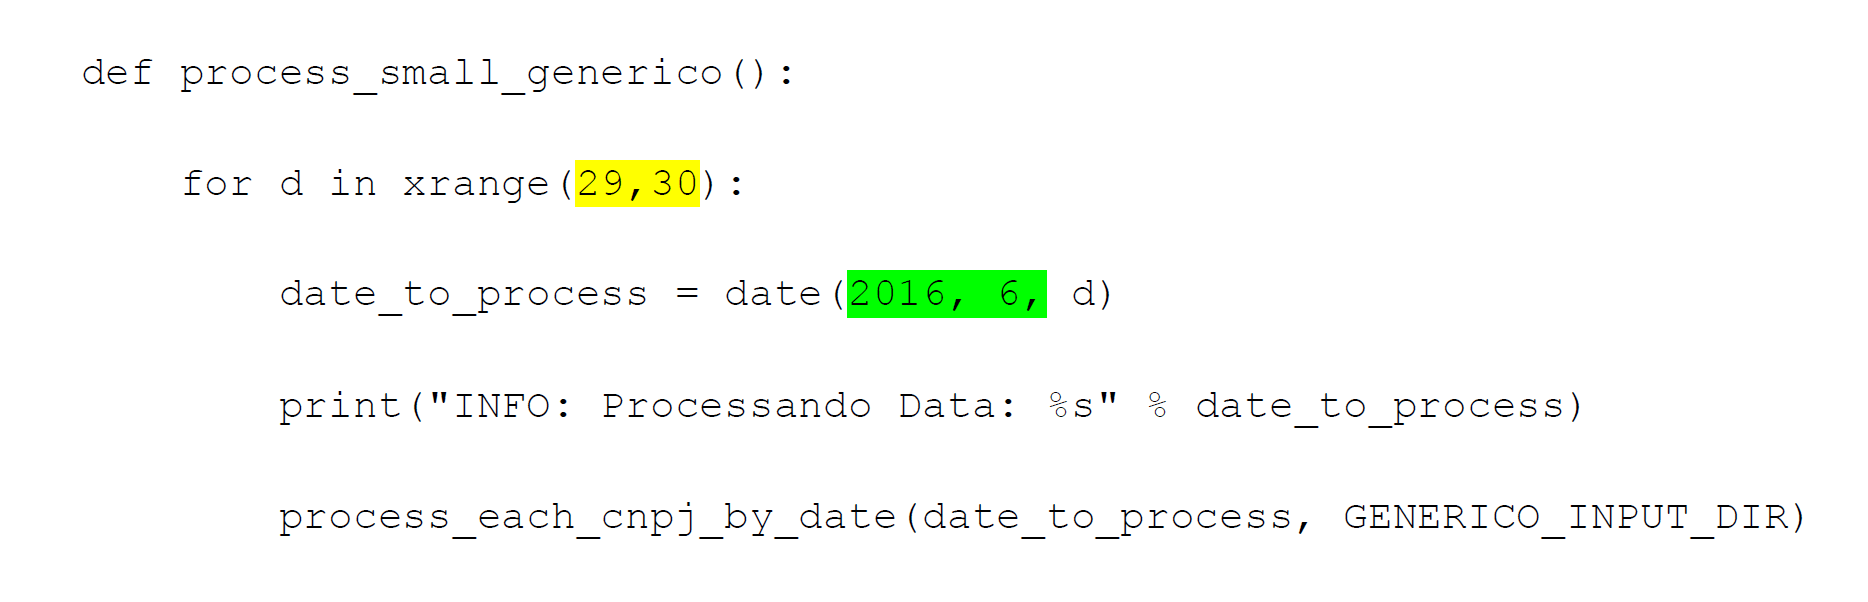
\includegraphics[width=1.0\textwidth]{genericos.png}
  \caption{Trecho de código a ser alterado}
    \label{fig:genericos}
\end{figure}

No exemplo da figura~\ref{fig:genericos} uma vez chamdo o $processa\_genericos.py$ pela linha de comando, processará \textbf{somente} o dia 29 do mês 6 de 2016.

Arquivos de logs com extensão \textbf{.log} serão gerados no mesmo diretório para auxiliar em caso de problemas.

O programa digere os dados da pasta \textbf{Cupons/processar (.NS)} e o resultado da digesão dos dados estarão na pasta \textbf{Cupons/processados (.csv, .pag).}.  \footnote{Obs. Sempre que possível cheque se a pasta a ser processada contém os arquivos coletados.}



\section{Sugestão de testes}

\begin{itemize}
    \item Reprocessamento dos arquivos de teste, para os equipamentos Daruma e SAT 
    \item Validação junto ao Banco de Dados.
\end{itemize}

\begin{thebibliography}{1}
  \bibitem{sat} {\em Especificação Técnica de Requisitos - SAT. pag. 96}  2016.
\end{thebibliography}

\end{document}               % End of document.